\documentclass{article}

\usepackage{amsmath,amssymb,geometry,tikz}
\usepackage{xepersian}

\setlength{\parindent}{0pt}
\setlength{\parskip}{3mm}

\newcounter{questionnumber}
\setcounter{questionnumber}{1}

\newcommand{\Q}{
\textbf{سوال \thequestionnumber)}
\stepcounter{questionnumber}
}

\newcommand{\eqn}[1]{
\begin{equation}\begin{split}
#1
\end{split}\end{equation}
}

\begin{document}
\LARGE
\begin{center}
\settextfont{IranNastaliq}

به نام زیبایی

%\begin{figure}[h]
%\centering
%\includegraphics[width=30mm]{kntu_logo.eps}
%\end{figure}

تمرینات سری هفتم درس احتمال مهندسی

\end{center}
\hrulefill
\large

\Q

فرض کنید در نقشه‌ی زیر قصد داریم از شهر A به شهر Z برویم. هر یک از 7 لینک نقشه‌ی زیر، با احتمال $p$ مستقل از سایر لینک ها سالم هستند. احتمال آن که مسیر سالمی از A تا Z وجود داشته باشد چقدر است؟

\begin{figure}[h]
\Large
\centering
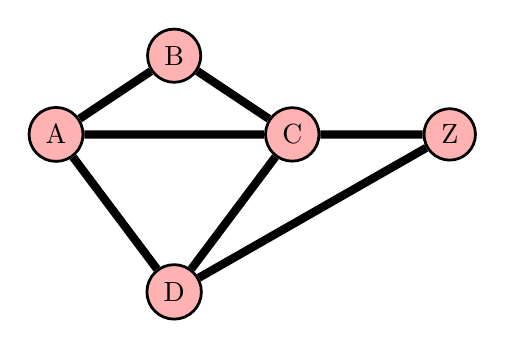
\begin{tikzpicture}
\node [draw=black,fill=white!70!red,circle,line width=1] (A) at (0,0) {A};
\node [draw=black,fill=white!70!red,circle,line width=1] (B) at (1.5,1) {B};
\node [draw=black,fill=white!70!red,circle,line width=1] (C) at (3,0) {C};
\node [draw=black,fill=white!70!red,circle,line width=1] (D) at (1.5,-2) {D};
\node [draw=black,fill=white!70!red,circle,line width=1] (Z) at (5,0) {Z};
\draw[line width=3]
(A)--(B)
(B)--(C)
(C)--(Z)
(A)--(C)
(A)--(D)
(D)--(C)
(D)--(Z)
;
\end{tikzpicture}
\end{figure}

\Q

یک سکه‌ی سالم را 10 بار پرتاب می‌کنیم.

الف) احتمال آن که دقیقا 3 بار شیر بیاید چقدر است؟

ب) احتمال آن که دست کم 2 بار خط بیاید چقدر است؟

پ) اگر بدانیم در 5 پرتاب اول خط آمده است، احتمال آن که در کل، دقیقا 7 بار خط آمده باشد چقدر است؟

\Q

یک تاس سالم را 6 بار پرتاب می‌کنیم.

الف) احتمال آن که جمع اعداد رو آمده در 6 پرتاب برابر 8 باشد چقدر است؟

ب) احتمال آن که در این 6 پرتاب، تمام اعداد 1 تا 6 ظاهر شوند چقدر است؟
\end{document}